\section{PKI and WoT}
\begin{figure}[H] %H为当前位置,!htb为忽略美学标准,htbp为浮动图形
    \centering %图片居中
    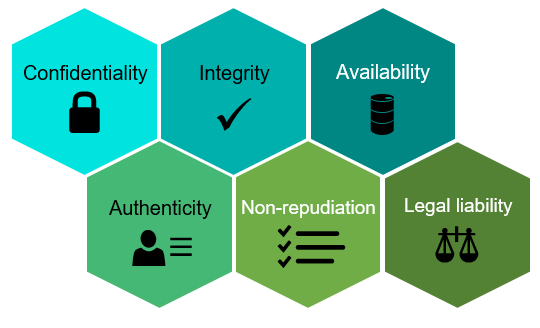
\includegraphics[width=0.3\textwidth]{figures/cia.png} %插入图片,[]中设置图片大小,{}中是图片文件名
    \caption{the basic cryptography security goals} %最终文档中希望显示的图片标题
    \label{Fig.2: the basic Cryptography Security goals} %用于文内引用的标签
\end{figure}
Before describing the two types of security systems, we need to understand the basic 
Cryptography Security goals, or CIA and the importance of public and private keys 
for cryptographic security\cite{b31}.
\begin{enumerate}[]
    \item \textbf{Confidentiality}: only entitled entities may be able to read the data.
    \item \textbf{Integrity}: tampering with a message will be detected.
    \item \textbf{Authenticity}: the communicating parties can be identified/verified.
\end{enumerate}
These are our core security goals. In addition, we might also have other goals:
\begin{enumerate}[]
    \item \textbf{Non-repudiation}: a communication partner cannot deny a message originated from her.
    \item \textbf{Forward secrecy}: compromise at this point in time does not lead to compromise of past connections.
    \item \textbf{Availability}: systems and data are available to individuals when they need it under any circumstances, including power outages or natural disasters.
\end{enumerate}
Attackers may listen in on messages in transit as well as manipulate them at will. An example
for a passive attack is eavesdropping: Alice sends Bob a message. Eve is listening on the line.
Thus, she can also see the message. Now she knows what Alice said. She eavesdropped on
Alice and Bob.


\subsection{PKI - Public Key Infrastructure}
One possible way of formalizing confidentiality is the Choice Plaintext Attack (CPA): 
an algorithm can provide confidentiality if a theoretical adversary is allowed to require 
the encryption of any plaintext and still not be able to obtain any information from the 
ciphertext\cite{b38}. Cryptography uses such models to analyze the security properties of a structure. 
CPA security algorithms provide encryption\cite{b31}.
\\
However, guarding against CPA does not help us defend against active attackers. Active 
attackers can manipulate messages. To prevent manipulation and forgery, we add authenticators 
to messages, such as message authentication tags\cite{b38}. The algorithm provides authenticity if 
the adversary is allowed to obtain the authentication tag of any message of its choice, 
but still cannot compute a valid authentication tag for the new message. This is called 
security under a chosen-ciphertext attack, which provides message authentication.
These security properties require certain assumptions that we will not discuss in detail 
here, such as the polynomial running time of the adversary and access to random bits.

\subsubsection{private-key cryptography}\cite{b38}
In the private key (symmetric) encryption setup, we assume that the communication partners 
have securely exchanged shared keys, one of which is typically 128 bits in length.
\\
A different key must be used for each direction of communication and for each purpose 
(e.g., encryption and authentication).
\begin{figure}[H] %H为当前位置,!htb为忽略美学标准,htbp为浮动图形
    \centering %图片居中
    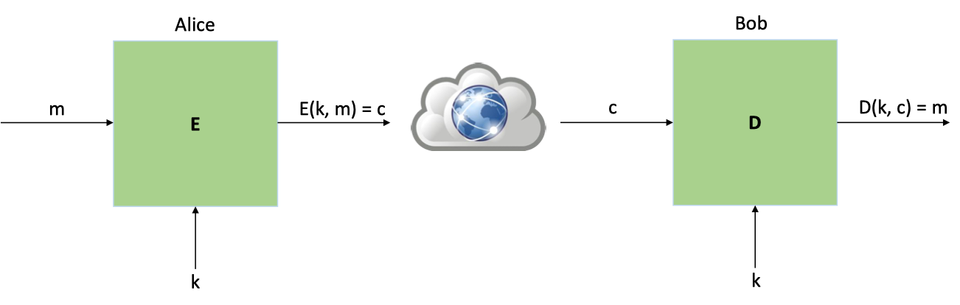
\includegraphics[width=0.5\textwidth]{figures/private.png} %插入图片,[]中设置图片大小,{}中是图片文件名
    \caption{private-key cryptography} %最终文档中希望显示的图片标题
    \label{Fig.2: private-key cryptography} %用于文内引用的标签
\end{figure}
We use encryption to provide confidentiality for the message m
\\
$k \ = \ Gen(1^n)$
\\
$c \ = \ Enc_k(m)$
\\
$m \ := \ Dec_k(c)$
\\
\\
Enc can be realized with functions such as AES-CTR or ChaCha20.
We use a message authentication code, e.g., HMAC-SHA2, to provide authenticity and 
integrity by generating a message authentication tag $t$ for a message m:
\\
$k \ = \ Gen(1^n)$
\\
$t \ = \ Mac_k(m)$
\\
$b \ := \ Vrfy_k(m, t)$
\\
\\
where $b$ can take both valid and invalid forms.
In order to obtain a reasonably expected level of security, we always want the message 
to have both: authenticated encryption.

\subsubsection{public-key cryptography}\cite{b38}
\\
We use public key (asymmetric) cryptography for three main purposes: confidentiality, 
authentication, and key exchange. In a public key scheme, each party has a key pair 
consisting of a private key $sk$ and a corresponding public key $pk$.
\begin{figure}[H] %H为当前位置,!htb为忽略美学标准,htbp为浮动图形
    \centering %图片居中
    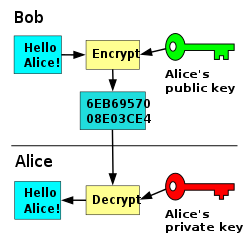
\includegraphics[width=0.3\textwidth]{figures/public_key.png} %插入图片,[]中设置图片大小,{}中是图片文件名
    \caption{public-key cryptography} %最终文档中希望显示的图片标题
    \label{Fig.2: public-key cryptography} %用于文内引用的标签
\end{figure}
Encryption is performed using the receiver's public key and decryption is performed 
by the receiver using his private key and vice versa.
\\
$(pk, sk) \ = \ Gen(1^n)$
\\
$c \ = \ Enc_{pk}(m)$
\\
$m \ := \ Dec_{sk}(c)$
\\
\\
Encryption algorithms can be based on RSA or ECDH issues, such as RSA-OAEP.
\\
Signatures are created using a private key and verified using the corresponding public key. 
They provide not only authenticity but also non-repudiation. Examples of signature algorithms 
are Ed25519 and RSA-PSS.
\\
$(pk, sk) \ = \ Gen(1^n)$
\\
$s \ = \ Sign_{sk}(m)$
\\
$b \ := \ Vrfy_{pk}(m, s)$
\\
\\
Because public-key encryption is typically slower than secret-key encryption, it is often 
used in handshakes to utilize key distribution properties and generate shared secret keys, 
which are then used to protect bulk traffic.
\\
Using cryptography correctly is only a small part of creating a secure system. Many things 
can still go wrong, such as side-channel attacks, buffer overflows, or other errors.
\\
It's easy to try to use cryptography to solve security problems, but the problems are often 
more complex and our assumptions ultimately prove invalid. Consider the following common problems:

\begin{enumerate}[]
    \item[*] side channels
    \item[*] inadequate threat model
    \item[*] replay attacks
    \item[*] traffic analysis
    \item[*] baseboard management controllers
    \item[*] correct behaviour is difficult for users
\end{enumerate}

\subsubsection{Signatures and Certificates}\cite{b38}
Digital signatures are the cyberspace version of handwritten signatures. Both digital and 
handwritten signatures are sent with the original data to provide authentication.
\begin{figure}[H] %H为当前位置,!htb为忽略美学标准,htbp为浮动图形
    \centering %图片居中
    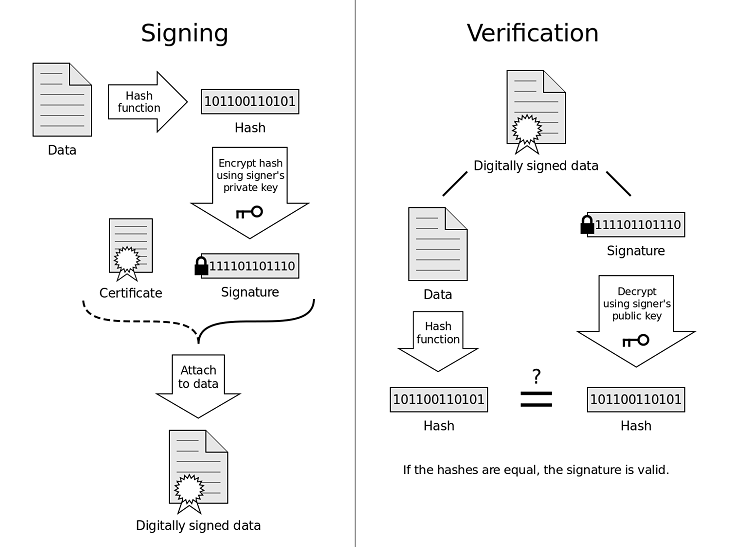
\includegraphics[width=0.5\textwidth]{figures/signature.png} %插入图片,[]中设置图片大小,{}中是图片文件名
    \caption{signatures and certificates} %最终文档中希望显示的图片标题
    \label{Fig.2: Signatures and Certificates} %用于文内引用的标签
\end{figure}
In addition, both are inseparable from the original data. In fact, the signature is not 
inextricably linked. They can be removed by simply cutting out the appropriate portion of 
the original document. However, this destroys the validity of the document.
\\
Handwritten signatures are usually placed at the bottom of the same sheet of paper that 
contains the data that the signer (Alice) wants to confirm in writing. Imagine that the 
situation would be different.
\\
Imagine a contract and a signature written on two different pieces of paper. This could 
be abused. For example, having the piece of paper with the signature, the recipient of the contract
signature (Bob) can reuse it to sign everything he wants (without asking Alice's permission).
\\
Let's return to digital signatures. Similar to the handwritten version, the digital 
signature sits after the original data. But instead of paper, we have packets and streams 
of data.
\\
In the context of TLS, however, we don't have contracts, only certificates, "which are 
data structures that bind public key values to subjects." (RFC 5280) More specifically, 
we have X.509 certificates here. The previous quote sounds rather complex and abstract, 
but it's actually not that difficult. The certificate for web server Bob (the subject) 
proves that Bob is the owner of the public key $K_{pubBOB}$ given in the certificate. 
Knowing this, Alice can determine one thing:
\\
Using $K_{pubBOB}$ to encrypt the data, only one person can decrypt and read the data.
\\
The owner of the corresponding private key $K_{privBOB}$. 
Assuming this key is stored securely, the only person who knows $K_{privBOB}$ is Bob. 
Therefore, by binding Bob to $K_{pubBOB}$, Alice can securely send data to Bob. It is 
important to understand these correlations. One question remains open. How does the binding happen?
\\
Now we can close the loop. 
Binding occurs through signatures. The signature is given by a trusted third party, 
thus confirming, "Yes, I know and guarantee that Bob and $K_{pubBOB}$ do belong together." 
The identity of that person and the mystery of trust in that context will be revealed 
on the next page, in "Public Key Infrastructure".
\\
But regarding trust in handwritten signatures, have you ever actually verified the 
signature of the person who signed the document you received. Imagine these three scenarios:
\begin{itemize}
    \item[*] Both parties to the contract were present when it was signed. This is similar to the situation where Alice physically walks to Bob's house and obtains Bob's public key.
    \item[*] Since Alice already has the document with Bob's signature, she can verify Bob's signature by comparing the two signatures on the two documents. This is equivalent to the case where Alice already knows Bob's public key.
    \item[*] Alice just believes that the signature is indeed signed by Bob. Otherwise someone is breaking the law. This is analogous to the case where Alice trusts a trusted third party who signed the certificate.
\end{itemize}

\subsubsection{Transport Layer Security}\cite{b38}
TLS stands for Transport Layer Security, a protocol used to protect Layer 4 traffic. 
While researching more about it, you may stumble upon the term SSL (Secure Sockets Layer), 
which is the predecessor to TLS.
\\
The Internet Engineering Task Force (IETF) released TLS 1.3 in August 2018. The version it 
replaces, TLS 1.2, was standardized a decade ago in 2008, but it is still widely deployed 
and is only slowly being replaced by its successor.
\begin{figure}[H] %H为当前位置,!htb为忽略美学标准,htbp为浮动图形
    \centering %图片居中
    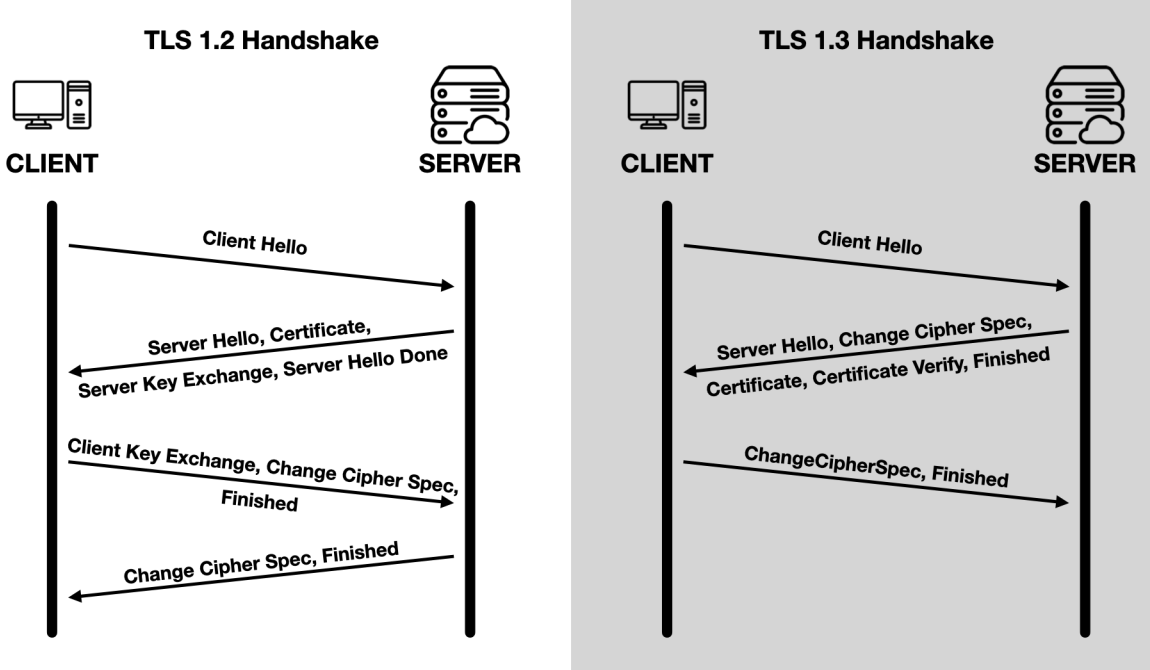
\includegraphics[width=0.5\textwidth]{figures/TLS.png} %插入图片,[]中设置图片大小,{}中是图片文件名
    \caption{TLS 1.2 and TLS 1.3 handshake} %最终文档中希望显示的图片标题
    \label{Fig.2: TLS 1.2 and TLS 1.3 handshake} %用于文内引用的标签
\end{figure}
The diagram above \ref{Fig.2: TLS 1.2 and TLS 1.3 handshake} briefly summarizes the 
TLS 1.2 and TLS 1.3 handshakes. You can see a 
representation of each of the 4 main segments of TLS 1.2 and the 3 segments of TLS 1.3.
\begin{enumerate}[]
    \item[*] Step 1: Client Hello
        \begin{enumerate}[]
            \item[*]  The Client hello message is a request to the server to begin a TLS handshake.
            \item[*] The message includes the client's TLS version, a random value, and a list of supported cipher suites.
        \end{enumerate}
    \item[*] Step 2: Server Hello
        \begin{enumerate}[]
            \item[*] After receiving the Client Hello message, the server will
                \begin{enumerate}[]
                    \item[*] confirm whether it supports the TLS version.
                    \item[*] choose a cipher suite from the list in the Client Hello message.
                    \item[*] generate a server random value.
                \end{enumerate}
                This information will be as a response to the client in a Server Hello message.
            \item[*] The server will also send the Certificate to the client.
            \item[*] Then the server will send the Server Key exchange.
            \item[*] In the end, a Server Hello Done message is sent to tell the client that all messages have been sent.
        \end{enumerate}
    \item[*] Step 3: Client Key Exchange
        \begin{enumerate}[]
            \item[*] After the client receives the server certificate, it will verify the 
            certificate and generate encryption keys using the client's and server's public key 
            and the two random numbers. Then the client sends a Change Cipher Spec message to 
            inform it that it changes to encrypted communication.
            \item[*] Then the client will send the Client Key exchange.
            \item[*] The client sends a Finished message to indicate it has completed its 
            part of the handshake.
        \end{enumerate}
    \item[*] Step 4: Server Change Cipher Spec
        \begin{enumerate}[]
            \item[*] After the server receives a Client Key Exchange message, it will use 
            it to compute the Master Key. Then, the server sends a Change Cipher Spec message 
            to inform it that it changes to encrypted communication.
            \item[*] Finally, a Finished message is sent to acknowledge that the key exchange 
            and authentication processes are finished successfully.
        \end{enumerate}
\end{enumerate}
\\
TLS 1.3 drops support for older, less secure cryptographic features. TLS 1.3 reduces 
TLS handshakes, 1-RTT instead of 2-RTT. In addition, the TLS 1.3 supports 0-RTT handshake 
which can be used, if client and server share a pre-shared key (either obtained externally 
or via a previous handshake). This allows the client to send data on the first flight.

\subsubsection{Diffie-Hellman-Key-Exchange}\cite{b38}
A fundamental problem when using symmetric keys is how to exchange them without anyone 
knowing or generating them, so that ultimately the two parties involved share the same 
key. One method of communicating without a secure channel is Diffie-Hellman-Key-Exchange.
\\
During the handshake, both parties agree on the parameters of the key derivation in the 
exchange message. Knowing them does not help an attacker understand the key. The basic 
principle of key derivation between Alice and Bob is the following scheme:

\begin{enumerate}[]
    \item[*] Alice and Bob agree on two parameters $g$ and $p$ for the key export. This can be done by Alice simply choosing them and sending them to Bob.
    \item[*] Both then generate a random number. This number is known only to them and will not be sent anywhere. Using this random number, Alice calculates $A \ = \ g^a \ mod \ p$ and Bob calculates $B \ = \ g^b \ mod \ p$. 
    $A$ and $B$ are then sent to their respective other partners.
    \item[*] They can now both generate the shared key K by computing $K \ = \ B^a \ mod \ p$ and $K \ = \ A^b \ mod \ p$.
\end{enumerate}
\\
Alice and Bob now share the same key $K$. The important thing here is that it is not possible 
to derive $K$ by knowing $g$, $p$, $A$, and $B$. For this, the attacker needs to keep the random numbers 
$a$ and $b$ secret.
By this algorithm it allows both parties to establish a key over an insecure channel without any prior information.

\subsubsection{Certificate Authority}\cite{b38}
There is still one question. Whose key is it? It is the public key of an 
organization called a Certificate Authority (CA). The CA issues the certificate and 
also signs it using its private key. The signing is actually performed by a 
Registration Authority (RA). In many cases, the CA also assumes the role of the RA. 
For the sake of clarity, we will consider here a CA that also signs the certificates 
it issues.
\\
We can only trust the server certificate if we can rely on the CA. Thus, we are 
simply transferring the trust issue to another entity. However, in PKI, CAs are 
trusted third parties, which means that we have no choice but to trust them or to 
obtain the server's public key on a different secure channel. We don't actually have 
to trust this particular CA. Each CA itself has a certificate, similar to the server's 
certificate. Our CA's certificate is signed by another CA's private key. Once again, 
we are transferring trust. What we have here is a chain of trust, the last link of which 
is the root CA. Since there is no CA above the root CA, there is no CA that can sign 
the root CA's certificate. It is "self-signed". In short, if you trust the root CA and 
find a gapless chain to the CA that signed the server's certificate, then you trust it. 
Usually, browsers provide a list of pre-installed trusted CAs.
\\
In Figure \ref{Fig.2: PKI_Chain_of_Trust}, you can see a graphical representation of 
such a chain of trust. A client requests a service from a server.
\\
Since it is a TLS-protected session, the client asks the server to prove its identity 
with a certificate. It is signed by a $CA_n$. The client has never heard of $CA_n$ and obtains 
a certificate from $CA_n$. It is signed by $CA_{n-1}$. Since the client only knows the root CA, 
it must obtain all certificates until it retrieves one signed by the root CA.

\begin{figure}[H] %H为当前位置,!htb为忽略美学标准,htbp为浮动图形
    \centering %图片居中
    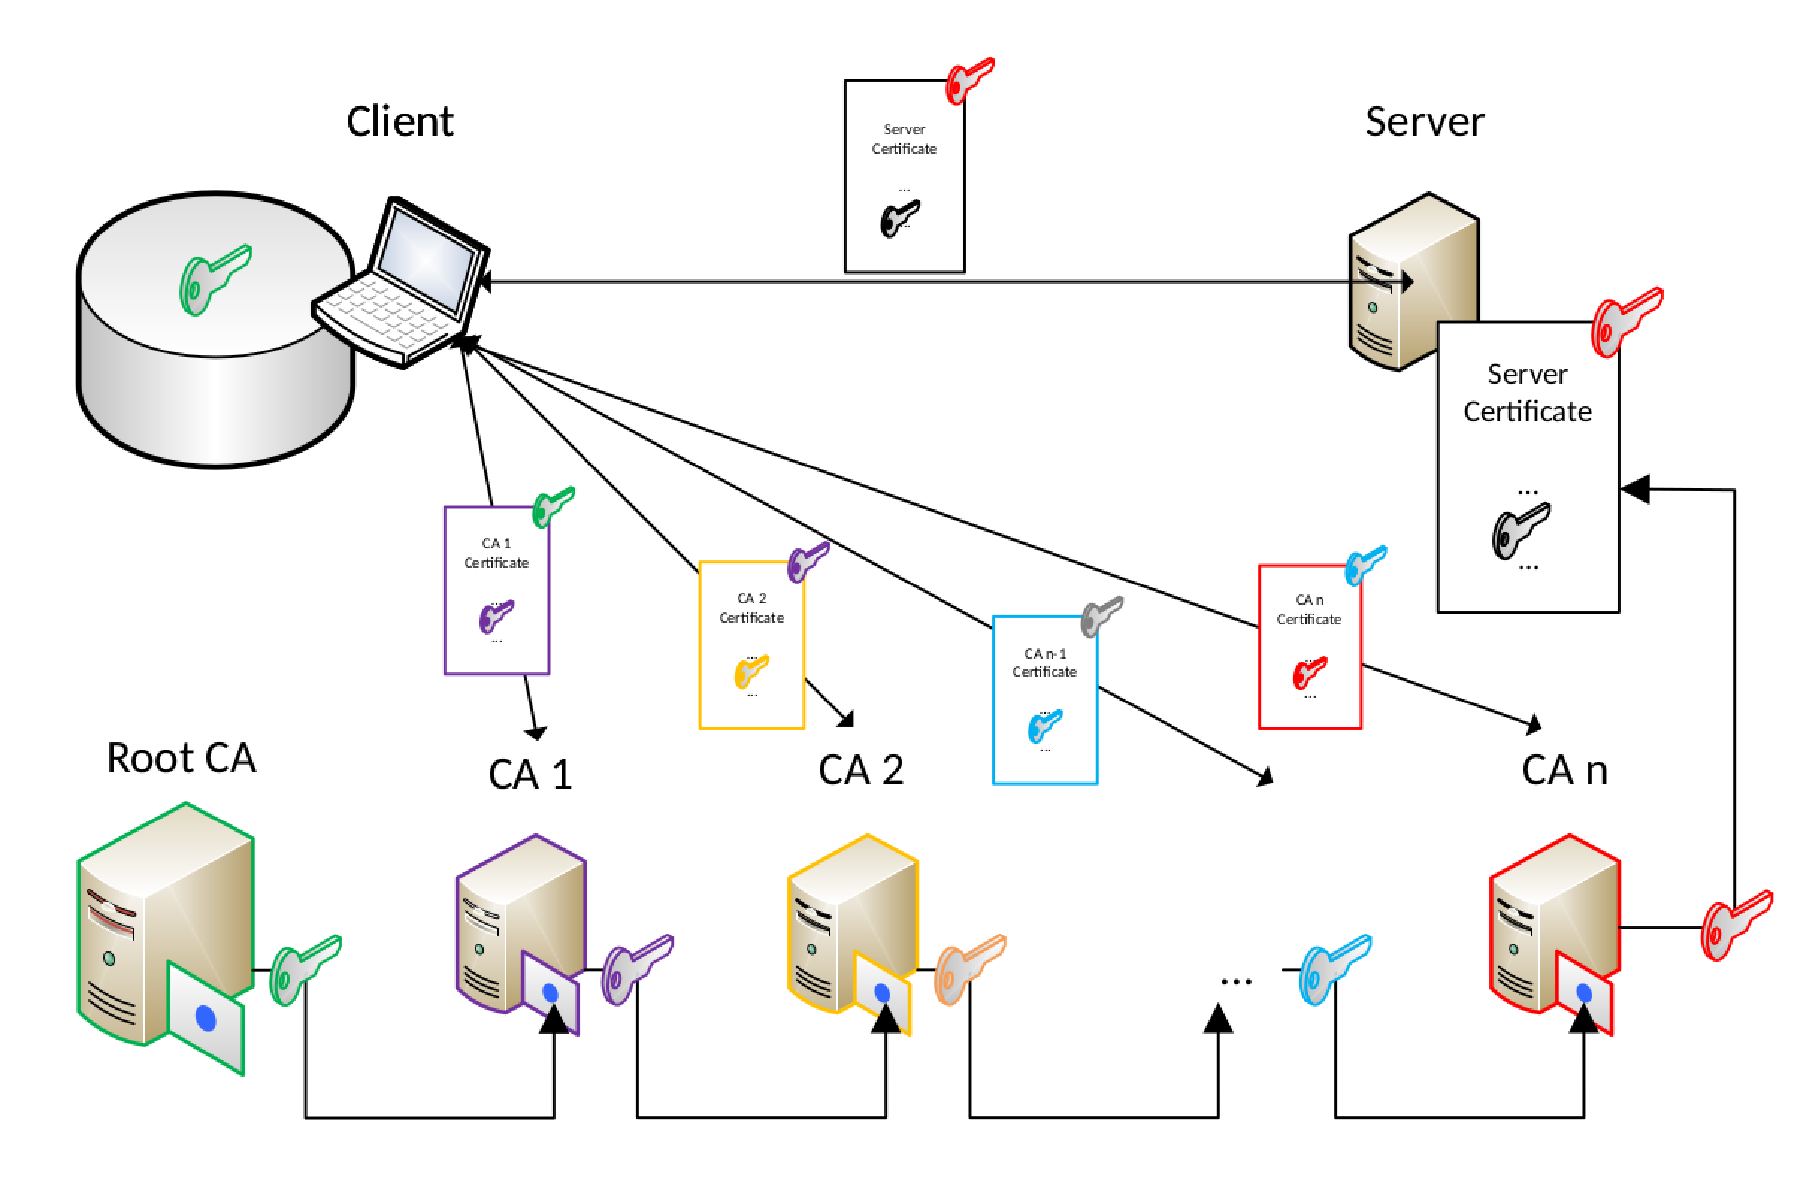
\includegraphics[width=0.5\textwidth]{figures/PKI_Chain_of_Trust.png} %插入图片,[]中设置图片大小,{}中是图片文件名
    \caption{PKI - Chain of Trust} %最终文档中希望显示的图片标题
    \label{Fig.2: PKI_Chain_of_Trust} %用于文内引用的标签
\end{figure}

\subsubsection{Certification Request}\cite{b38}
Let's consider a server. Before it can prove its identity with a signed certificate, it must 
retrieve one. The certificate binds the identity inextricably to the public key. In addition 
to its identity (e.g., company name) and its proprietary name (domain name, e.g., 
"www.example.com"), the server needs the public key to be used for the certification request 
(CR or certificate signing request CSR). The key pair is generated locally by the server 
and the corresponding private key is kept secret. After all the information has been 
collected, the data is packaged into the authentication request, e.g. in PKCS#10 format. 
To prove that it knows the corresponding private key, the server must sign the CSR. Upon 
receipt of the request, the CA must validate the CSR. This can be done in a number of ways, 
such as forcing the requester to present a passport (although this is less stringent in 
most cases). Once the CSR is verified, the CA issues a signing certificate (e.g., an X.509 
certificate).


\subsection{WoT - Web of Trust}
Web of Trust (WoT)\cite{b7} is a concept in cryptography that can be used to authenticate the 
identity of the holder of a public key, as applied in PGP, GnuPG, or other OpenPGP-compatible 
systems\cite{b8, b9, b10}. Trust networks use the concept of decentralization, unlike public key 
infrastructures that rely on digital certificate certification authorities. In a 
computer network, there can be many independent trust networks at the same time, and 
any user can be a part of one of these networks, or a link between different networks\cite{b11}.
\\
In PKI, all trust stems from trust in the CA organization, but CA organizations can make 
mistakes. Even those CA organizations that have not made any errors so far, there is 
no guarantee that they will not make errors in the future. In contrast to PKI, where 
there is unconditional trust in CAs, another type of PKI is called a "network of trust", 
where there are no CAs, but rather a network built on one-to-one trust\cite{b7}.

\begin{figure}[H] %H为当前位置,!htb为忽略美学标准,htbp为浮动图形
    \centering %图片居中
    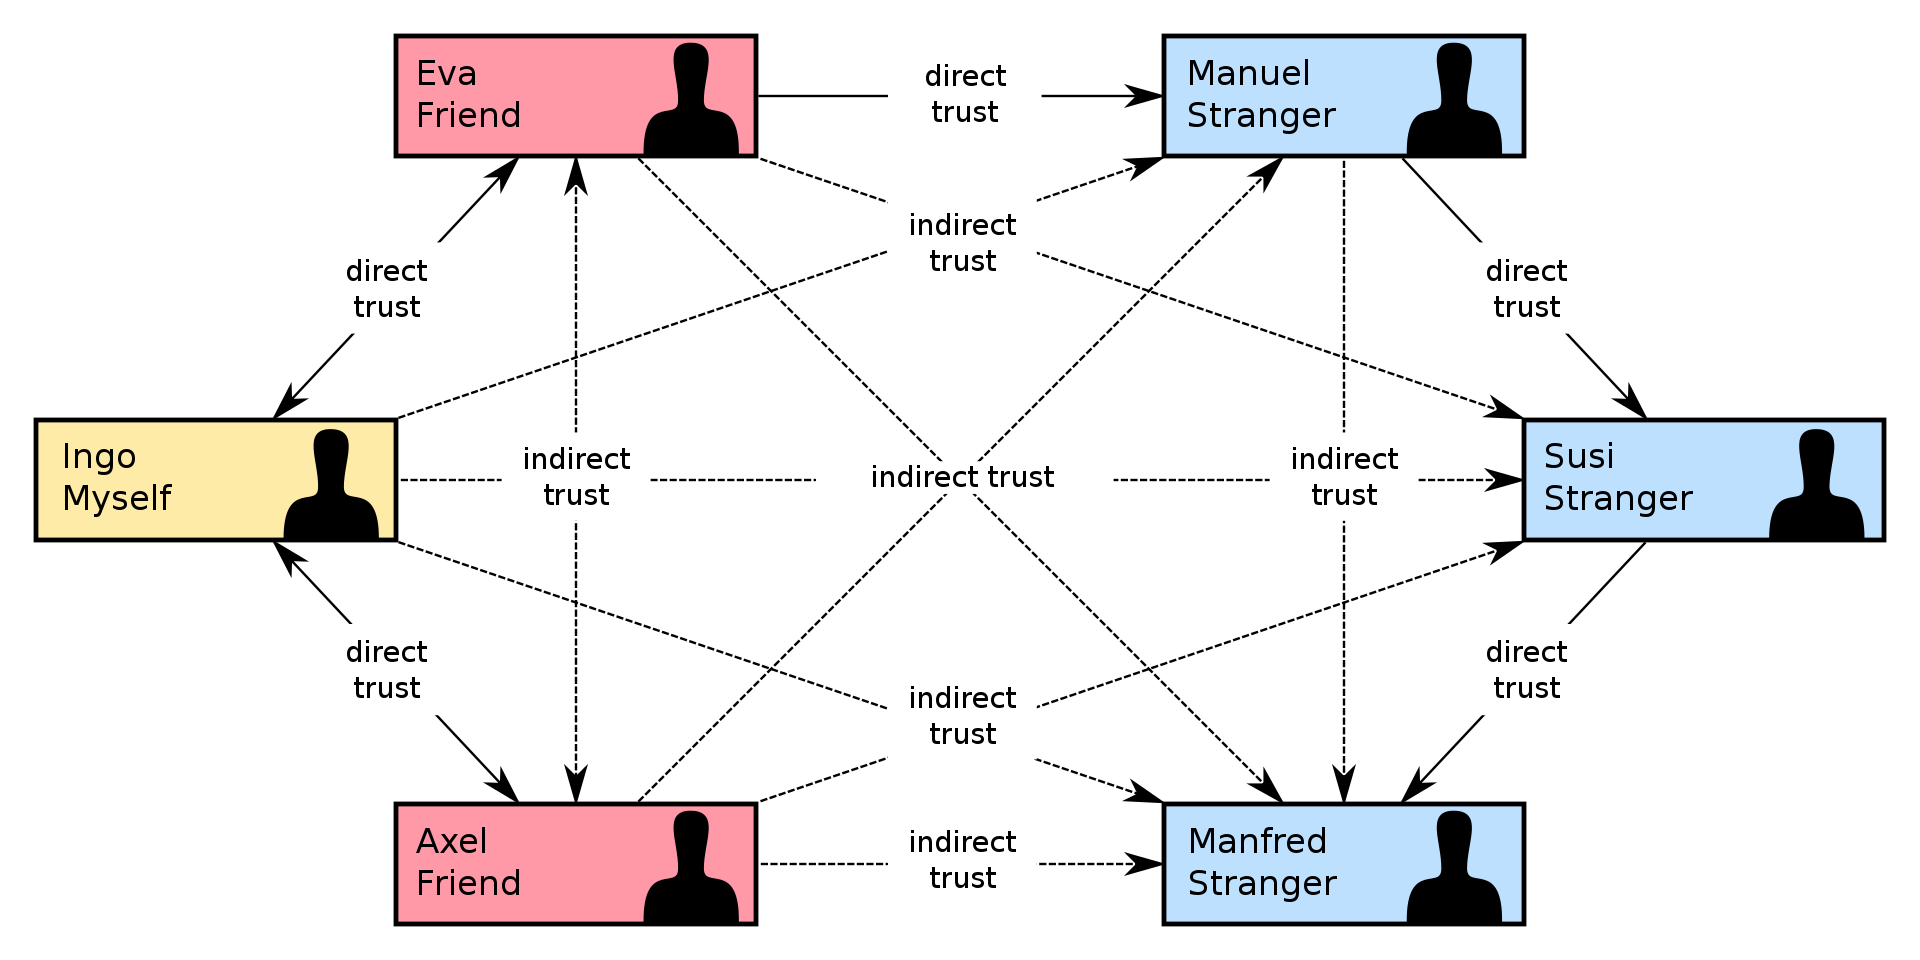
\includegraphics[width=0.5\textwidth]{figures/decentralized_trust_model.png} %插入图片,[]中设置图片大小,{}中是图片文件名
    \caption{The decentralized trust model} %最终文档中希望显示的图片标题
    \label{Fig.2: decentralized_trust_model} %用于文内引用的标签
\end{figure}

The concept of trust networks was first introduced by PGP author Philip Zimmermann in 
the PGP 2.0 manual\cite{b7}.
\\
Over time, you will gradually collect many other people's keys, some of whom you may 
be willing to sign up to trust (treating them as trusted introducers). Other people 
will also sign up for some other people's keys that they themselves trust (choosing 
their own trusted introducers).
\\
Each person gradually accumulates a number of keys that have been signed and trusted 
by others, and then signs and distributes them himself. Then one can expect that the 
next person to get the key will always have one or two people on the signing list that 
he or she trusts. This eventually creates a distributed, cheat-proof trust network of 
all public keys.
\\
This is the idea of trust in a network of trust. When any user uses someone else's 
public key, he becomes a referrer of that public key. When such a procedure is 
continued, a network of trust is formed where all public keys are decentralized 
and fault-tolerant.

\begin{figure}[H] %H为当前位置,!htb为忽略美学标准,htbp为浮动图形
    \centering %图片居中
    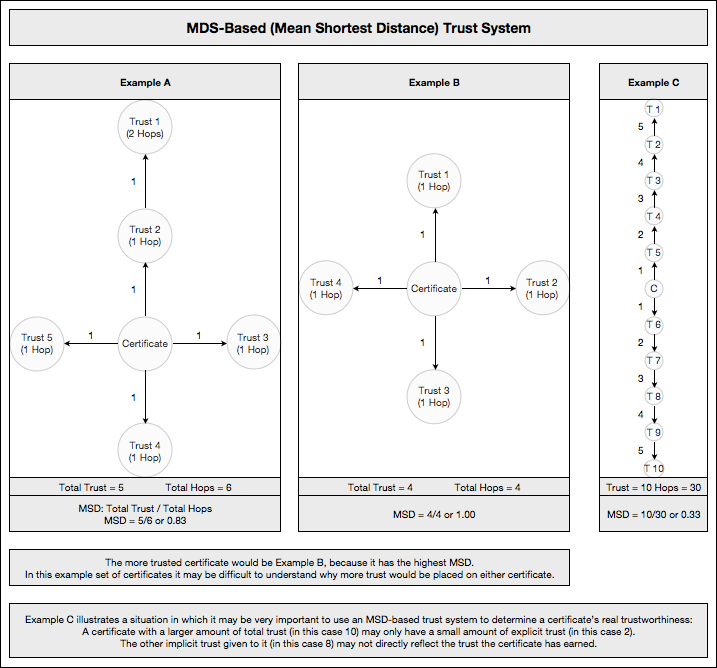
\includegraphics[width=0.5\textwidth]{figures/trustSystem.png} %插入图片,[]中设置图片大小,{}中是图片文件名
    \caption{MDS-Based (Mean Shortest Distance) Trust System} %最终文档中希望显示的图片标题
    \label{Fig.2: MDS-Based (Mean Shortest Distance) Trust System} %用于文内引用的标签
\end{figure}

In a trust network, any trust network user can verify the public key credentials of other 
trust network users. However, such credentials are only trusted if the third party also 
considers the verifier to be a trusted referrer. (That is, if you want to trust a key that 
I think is valid, you have to recognize me as a trusted referrer. Otherwise my validation 
for another key is meaningless to you.)
\\
What is stored in each user's public keystore contains the following information:
\\
Whether a key is considered valid by the user.
\\
The degree to which the user trusts that key, which relates to the key owner's 
ability to be a verifier of other keys.
\\
You point out the counts on my comment based on my copy of the key.
\\
It's really a reputation system: some people have a good reputation for being 
trusted, and people thus trust that their verification of other keys is valid.

\subsubsection{Direct Trust}
Direct trust is the simplest model of trust. In this model, the user trusts a 
key to be valid because they know where it came from\cite{b27}. All cryptosystems use this 
form of trust to some extent. For example, in web browsers, CA agency root 
certificates are trusted directly because they are built or embedded into the operating system 
or the browsers\cite{b28}.

\begin{figure}[H] %H为当前位置,!htb为忽略美学标准,htbp为浮动图形
    \centering %图片居中
    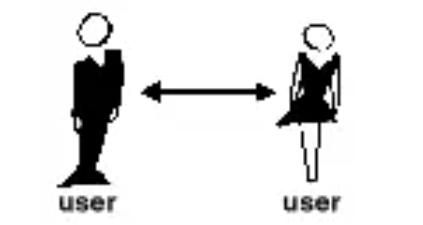
\includegraphics[width=0.2\textwidth]{figures/directTrust.png} %插入图片,[]中设置图片大小,{}中是图片文件名
    \caption{Direct Trust} %最终文档中希望显示的图片标题
    \label{Fig.3: Direct Trust} %用于文内引用的标签
\end{figure}


\subsubsection{Trust Tree}
In the chain of trust, there will be a number of trusts extended from the "root 
certificate". These certificates may vouch for themselves, or vouch for certificates 
at lower levels. Think of this as a chain of trust\cite{b31}. The authenticity of a downstream 
certificate is proven by the authenticity of the certificate that issued it, until 
it is directly trusted by the root certificate. From an individual perspective, this 
is a chain of trust, while from a holistic perspective, it is actually a tree of trust\cite{b28}.

\begin{figure}[H] %H为当前位置,!htb为忽略美学标准,htbp为浮动图形
    \centering %图片居中
    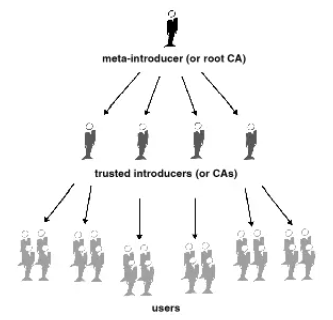
\includegraphics[width=0.4\textwidth]{figures/trustTree.png} %插入图片,[]中设置图片大小,{}中是图片文件名
    \caption{Trust Tree} %最终文档中希望显示的图片标题
    \label{Fig.4: Trust Tree} %用于文内引用的标签
\end{figure}


\subsubsection{Trust Network}
A trust network differs from the above two models in that a trust network can be 
thought as a combination of the direct trusts and trust trees. In a trust 
network\cite{b27}, you believe that a key is real because someone you trust believes it to 
be real. This person is called the introducer\cite{b28}.
\\
You may have heard of the Six Degrees of Separation theory\cite{b37}: that any two people 
in the world who don't know each other need up to six intermediaries to be able 
to make a connection\cite{b29}.
\begin{figure}[H] %H为当前位置,!htb为忽略美学标准,htbp为浮动图形
    \centering %图片居中
    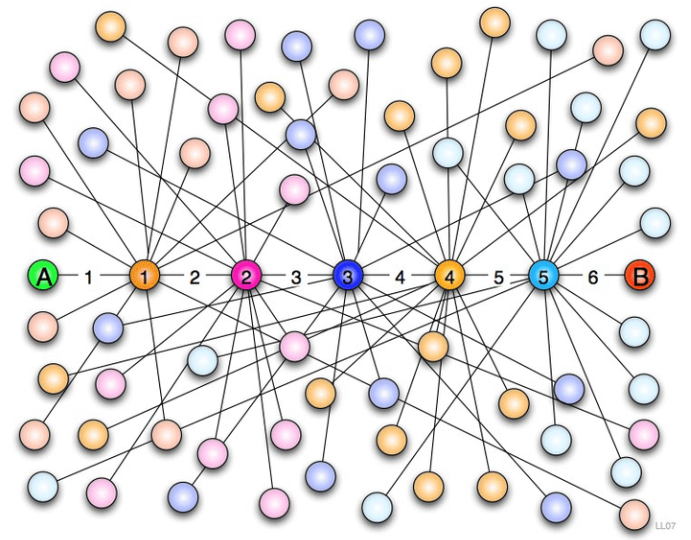
\includegraphics[width=0.4\textwidth]{figures/trustNet.png} %插入图片,[]中设置图片大小,{}中是图片文件名
    \caption{Trust Network} %最终文档中希望显示的图片标题
    \label{Fig.5: Trust Network} %用于文内引用的标签
\end{figure}


\subsubsection{PGP}
The Pretty Good Privacy (PGP) PGP is a family of software systems
developed by Philip R. Zimmermann from which OpenPGP is based. It is 
one such security protocol based on 
a network of trust\cite{b11}.The biggest difference between PGP and other security protocols 
is the way he verifies the certificates - based on a network of trust, instead of PKI 
and root certificates\cite{b12}.
\\
In PGP, there are three levels of trust for a key:

\begin{enumerate}[]
    \item \textbf{Full Trust (or Complete Trust)}
    \item \textbf{Half Trust (or Suspicion)}
    \item \textbf{Distrust (or Complete Distrust or lack of trust)}
\end{enumerate}
\\
Only a key that is fully trusted by one referrer, or half-trusted by two referrers, 
can be determined to be a valid key.

\begin{figure}[H] %H为当前位置,!htb为忽略美学标准,htbp为浮动图形
    \centering %图片居中
    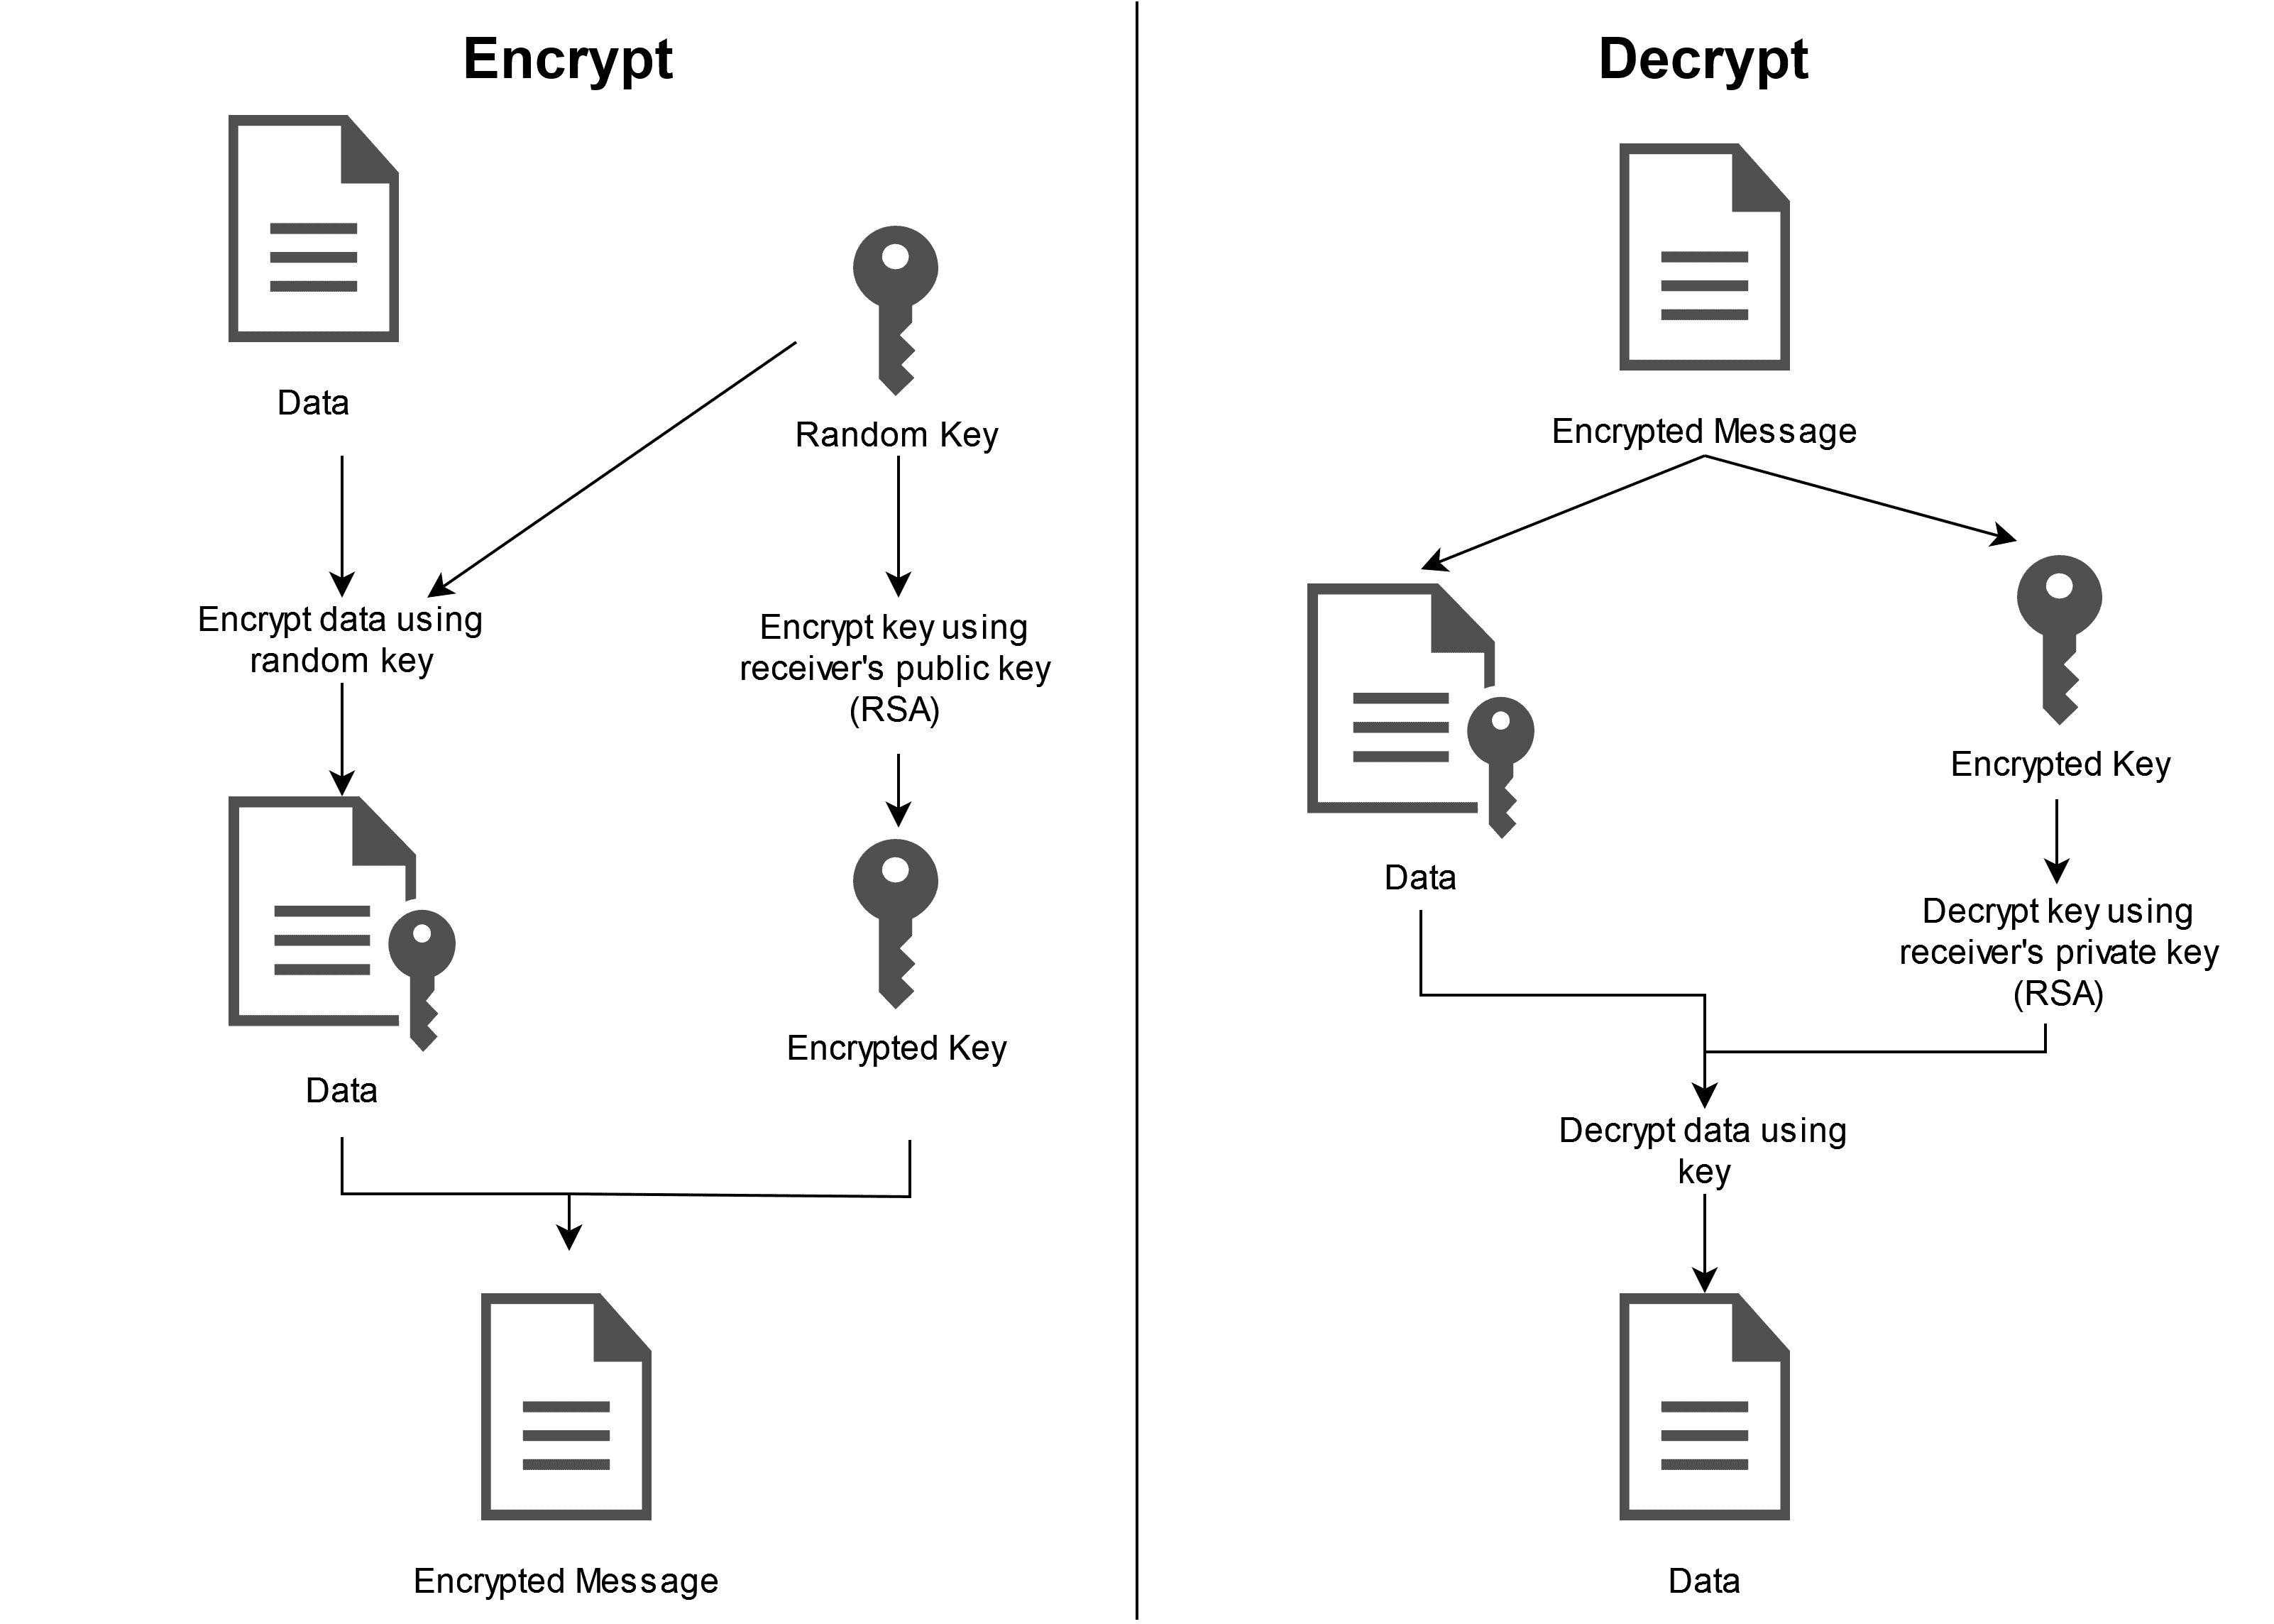
\includegraphics[width=0.5\textwidth]{figures/PGP.png} %插入图片,[]中设置图片大小,{}中是图片文件名
    \caption{PGP} %最终文档中希望显示的图片标题
    \label{Fig.6: PGP} %用于文内引用的标签
\end{figure}

Using the commonly used encrypted email as an example, the exact 
workflow is:
\\
Alice wants to send an email to Bob.
\begin{enumerate}[]
    \item Bob generates a pair of keys (public and private) and sends 
    the public key to Alice.
    \item The PGP protocol uses an algorithm to generate a randomized 
    session key, which is a very large number and is used only once.
    \item Alice encrypts the email, using the key she just generated, 
    and encrypts that key using Bob's public key.
    \item Finally, Alice sends the encrypted email and the key to 
    Bob, who decrypts it using his own private key to get the 
    session key, which in turn allows him to decrypt the complete email.
\end{enumerate}
\\
In PGP, we no longer rely on CA organizations to help us check the authenticity of 
certificates, we only trust our own judgment. The concept of decentralization embedded 
in it will bring us more reliable and secure encrypted communication\cite{b12}.


\subsubsection{Advantages and Disadvantages of PGP}
PGP encryption has the following advantages:\cite{b9}
\begin{enumerate}[]
    \item Secure: PGP encryption uses strong encryption algorithms to protect data.
    \item Reliable: PGP encryption prevents data from being read or modified by unauthorized users.
    \item Flexible: PGP can be used to encrypt and authenticate emails, files and other data.
\end{enumerate}
\\
PGP encryption has the following disadvantages:\cite{b9}
\begin{enumerate}[]
    \item Complexity: The use of PGP encryption can be complex.
    \item Performance: PGP encryption may affect the performance of data transmission.
\end{enumerate}

\subsubsection{Applications of PGP Encryption}
PGP has three main uses\cite{b9}:
\begin{enumerate}[]
    \item Communication security, such as encrypted e-mail and file sharing.
    \item Online transactions, such as online banking and e-commerce.
    \item Protect sensitive data such as financial information, medical records and legal documents.
\end{enumerate}
    
Of these, sending and receiving encrypted e-mail is the primary 
application of PGP.\cite{b7} Digital signatures are a technology based on 
public key encryption used to prove the identity of the sender 
of a message and the integrity of the message, as well as to 
prevent the message from being tampered with.
\\
The sender encrypts the digest of the message using his 
private key to generate a digital signature. The receiver 
decrypts the digital signature using the sender's public 
key and generates a digest of the message, comparing the 
two digests for consistency to verify the integrity and 
identity of the message. If the digital signature verification 
fails, the message may have been tampered with or come from a 
forged sender.\cite{b7}
\\
PGP uses symmetric encryption algorithms to protect data 
confidentiality. It uses public key encryption algorithms to protect 
the security of symmetric keys. In addition, it uses digital signature 
techniques to verify the integrity and identity of messages. 
This combination of symmetric key and public key encryption 
strikes a balance between security and efficiency. PGP has become 
a widely used standard for data encryption and digital signatures, 
protecting user privacy and security\cite{b7, b9, b36}.
\\
One might also ask: how can one securely get the public key of an intermediary or other 
friends? It is indeed possible that a user gets the public key of some other friend that 
is a fake. But this would require that the evildoer must have earned the trust of many 
people in the web of trust. This is unlikely, since it would have to be planned over a 
long period of time.
\\
Of course, the PGP has a preventive proposal for this possibility, which is to have a 
generally trusted organization take on the role of notary public, which is called a 
certification authority. Every public key signed by it is considered valid, so that everyone 
just has to have its public key. It is convenient to authenticate its public key because 
it provides this service widely. It is extremely difficult to fake its public key since 
it is widely available.\cite{b8, b10} Such a cryptographic system that combines centralization and 
decentralization is a much better solution.

\subsubsection{GunPG command}
GnuPG is installed by default on all Linux distributions.\cite{b40, b41}
\\
GnuPG is free software designed to follow the OpenPGP technology standard set by the 
IETF and is compatible with PGP. GnuPG can be used to encrypt and sign communications 
and manage keys for asymmetric cryptography. GnuPG offers the following features:
\begin{enumerate}[]
    \item Public Key Encryption: GnuPG uses public key encryption to protect data from unauthorized access. 
    The public key is public, while the private key is private.
    \item Digital Signatures: GnuPG uses digital signatures to verify the integrity and 
    origin of files. Digital signatures are generated using a private key and can be verified 
    using a public key.
    \item Web of Trust: GnuPG uses a web of trust to determine the identity of 
    other users. A web of trust is a system where users sign each other's names to 
    establish a relationship of trust.
    \item Key Management: GnuPG provides a key management system to store and manage your keys.
\end{enumerate}
\\
Management logic for gpg key:\cite{b40, b41}
\begin{enumerate}[]
    \item Public Key Encryption: GnuPG uses public key encryption to protect data from unauthorized access. 
    The public key is public, while the private key is private.
    \item Digital Signatures: GnuPG uses digital signatures to verify the integrity and 
    origin of files. Digital signatures are generated using a private key and can be verified 
    using a public key.
    \item Web of Trust: GnuPG uses a web of trust to determine the identity of 
    other users. A web of trust is a system where users sign each other's names to 
    establish a relationship of trust.
    \item Key Management: GnuPG provides a key management system to store and manage your keys.
\end{enumerate}

\lstset{language=C}
\begin{lstlisting}
# Generate a master key
# step 0
gpg --full-gen-key

# step 1
gpg (GnuPG) 2.2.27; Copyright (C) 
2021 Free Software Foundation, 
Inc.
This is free software: you are 
free to change and redistribute 
it.
There is NO WARRANTY, to the 
extent permitted by law.

Please select what kind of key 
you want:
   (1) RSA and RSA (default)
   (2) DSA and Elgamal
   (3) DSA (sign only)
   (4) RSA (sign only)
  (14) Existing key from card
Your selection?
# default 1

# step 2
RSA keys may be between 1024 
and 4096 bits long.
What keysize do you want? (3072)
# Enter your desired key length 
# here, which should not be less 
# than 2048 bits for RSA.
# Of course, the higher the number 
# you enter, the more secure it will 
# be.
# Accordingly, the slower the 
# encryption and decryption will be.

# step 3
Please specify how long the key 
should be valid.
         0 = key does not expire
      <n>  = key expires in n days
      <n>w = key expires in n weeks
      <n>m = key expires in n months
      <n>y = key expires in n years
Key is valid for? (0) 
# By default, you can select 0, 
# which means it will never expire.
# You can change your expiration 
# time anytime before the expiration 
# date to make sure 
# you still have control over the 
# key.

# step 4
Key expires at Wed 11 Jan 2024 
05:50:53 PM CST
Is this correct? (y/N) y

# step 5
GnuPG needs to construct a user 
ID to identify your key.

Real name:  yyyyy
# It can be any name, so don't 
# enter your real name if you're 
# concerned about privacy.
Email address: yyyyy@gmail.com  
Comment:     # can be left blank
# If you don't want to use PGP to 
# authenticate your Git logs, you 
# can enter whatever you want here, 
# it doesn't even have to be a real 
# email address, it just has to be 
# known by the person who 
# receives your information. Privacy 
# is a serious issue, and once you 
# set it up and publish 
# it to a public key server, you 
# cannot delete it!


# step 6
You selected this USER-ID:
    "yyyyy <yyyyy@gmail.com>"

Change (N)ame, (C)omment, (E)mail 
or (O)kay/(Q)uit? o
# After confirming that there are 
no errors, enter o


# step 7
┌───────────────────────────────
│ Please enter the passphrase to 
│ protect your new key           
│                                
│ Passphrase: __________________
│                                
│       <OK>       <Cancel>     
└───────────────────────────────
# Enter a complex password and confirm.

# step 8
We need to generate a lot of random 
bytes. It is a good idea to perform
some other action (type on the keyboard,
move the mouse, utilize the
disks) during the prime generation; 
this gives the random number
generator a better chance to gain 
enough entropy.
# Randomize the movement of your mouse, 
# the more random your key is the more 
# secure it is.

# step 9              
gpg: key 99F583119B7E31F1 marked as 
ultimately trusted
gpg: revocation certificate stored 
as '/root/.gnupg/opegp-revocs.d/7053
58AB85366CAB05C0220F99F583599B7E31F1.rev'
public and secret key created and signed.

pub   rsa3072 2024-01-11 [SC]
      705358AB85366CAB05C0120F99F583599B
      7E31F1			 # your key id
uid   yyyyy <yyyyy@gmail.com>
sub   rsa3072 2024-01-11 [E]
# This is an automatically generated 
# subkey for encryption, the E stands
# for Encrypt.

\end{lstlisting}
\\
\\
The following are common abbreviations:\cite{b40, b41}
\\
A    =>    Authentication
\\
C    =>    Certify
\\
E    =>    Encrypt
\\
S    =>    Sign
\\
?    =>    Unknown capability
\\
sec  =>    Secret Key
\\
ssb  =>    Secret SuBkey
\\
pub  =>    Public Key
\\
sub  =>    Public Subkey
\\
\\
Other commands:\cite{b40, b41}
\begin{enumerate}[]
    \item import key: \\gpg --import \$\{filename\}.[pub|priv].gpg
    \item export public key: \\gpg --export -a \$\{keyid\} > \$\{filename\}.pub.gpg
    \item export secret key: \\gpg --export-secret-key -a \$\{keyid\} > \$\{filename\}.priv.gpg
    \item delete public key: \\gpg --delete-key \$\{keyid\}
    \item delete secret key: \\gpg --delete-secret-key \$\{keyid\}
    \item Backup and Restore gpg:
\end{enumerate}
\lstset{language=Python}
\begin{lstlisting}
#backup
gpg -a --export ${keyid} > public.gpg
gpg -a --export-secret-keys ${keyid} 
> private.gpg
gpg --export-ownertrust > ${keyid}-
ownertrust-gpg.txt

#restore
gpg --import private.gpg
gpg --import-ownertrust ${keyid}-
ownertrust-gpg.txt
\end{lstlisting}